%!TEX root = ../main.tex
% =============================================================
%  CAPÍTULO 4 — MARCO TECNOLÓGICO       (Entrega 4 · 10 % · 25/8)
% =============================================================

\chapter{Marco tecnológico}\label{cap:marco-tecnologico}

\begin{guia}[Guía de la cátedra: qué se evalúa en este capítulo]
Documenta el \emph{cómo}. No es un manual de uso: es la justificación
de cada elección tecnológica. Regla: nada ``porque sí''.
\begin{enumerate}
    \item \textbf{Arquitectura}: diagrama con componentes y conexiones,
          responsabilidad y tecnología de cada uno, flujo de datos y
          justificación del estilo arquitectónico con alternativas
          evaluadas (Sommerville, 2016).
    \item \textbf{Prototipo o \gls{g:mvp}}: cuál es y por qué; alcance
          implementado vs.\ simulado; capturas o enlace; cómo se probó.
    \item \textbf{Stack}: por tecnología, nombre, versión, capa, por qué
          (madurez, comunidad, costo, conocimiento del equipo) y qué
          alternativas se descartaron.
    \item \textbf{Infraestructura y base de datos}: dónde se aloja cada
          componente, escalabilidad, costos (enlazados al
          capítulo~\ref{cap:economica}), motor y modelo de datos.
    \item \textbf{Diseño y \gls{ux}}: quién lo usa, mockups, decisiones de
          diseño y \textbf{cómo se validó con usuarios} (la cátedra lo marca
          como importante; cuestionario en el apéndice~\ref{apx:encuesta}).
    \item \textbf{Seguridad, calidad y despliegue}: autenticación, control
          de acceso, cifrado, plan de pruebas, repositorio, \gls{cicd} y
          monitoreo.
\end{enumerate}
\end{guia}

\section{Arquitectura del sistema}\label{sec:n4.1}

El sistema se diseñó como un pipeline por etapas sucesivas y desacopladas. Esta estructura modular permite que cada componente cumpla un rol único dentro del procesamiento: el análisis sintáctico genera el AST, los constructores crean los nodos y aristas de la representación intermedia, y el motor de taint opera sobre el grafo final. La división simplifica además la estrategia de pruebas, ya que permite aislar y validar cada fase mediante pruebas unitarias independientes sin necesidad de ejecutar el pipeline completo para verificar un módulo interno.

La decisión se refleja además en la estrategia de pruebas. Al ejecutar la suite de tests, cada etapa se valida de forma independiente, lo que permite identificar con precisión en qué componente del pipeline se produce una falla. Una arquitectura monolítica impediría este nivel de aislamiento, dado que mezclaría el análisis sintáctico con el análisis semántico y forzaría a probar el sistema como una unidad indivisible.

\subsection{Organización en paquetes}\label{sec:n4.1.1}

El proyecto se organiza como un monorepo gestionado mediante espacios de trabajo de npm, compuesto por dos paquetes con responsabilidades diferenciadas. El paquete de núcleo concentra la totalidad del motor de análisis: análisis sintáctico, construcción de la representación intermedia, generación del grafo y detección de recorridos vulnerables. El paquete de visualización implementa la interfaz web y consume los resultados producidos por el núcleo, que expone además un punto de entrada sin dependencias de Node.js para ejecutar el mismo motor en el navegador. Esta separación permite que el motor de análisis opere de manera independiente de cualquier interfaz gráfica.

\subsection{Flujo de procesamiento}\label{sec:n4.1.2}

El procesamiento se inicia con los archivos fuente que el usuario selecciona en la versión web o indica en la interfaz de línea de comandos. Cada archivo es transformado en un árbol de sintaxis abstracta. A partir de dicho árbol se construye una representación intermedia compuesta por nodos tipados. Sobre esa representación operan tres constructores de aristas que se ejecutan de manera independiente sobre el mismo conjunto de nodos: el generador del grafo de llamadas, el analizador de flujo de datos intra-procedural y el analizador de flujo inter-procedural. La unión de los nodos y de las aristas producidas por los tres constructores conforma el grafo dirigido que constituye la representación central del programa. A continuación, la etapa de enlace entre archivos resuelve las llamadas a funciones importadas desde otros archivos del proyecto y agrega las aristas de invocación y de asociación de argumentos correspondientes, de modo que los grafos de los archivos conectados por llamadas se unen en un único grafo. Sobre dicho grafo opera el motor de análisis de contaminación, cuyos resultados se presentan en el módulo de visualización o en los reportes de la interfaz de línea de comandos.

\begin{figure}[H]
    \centering
    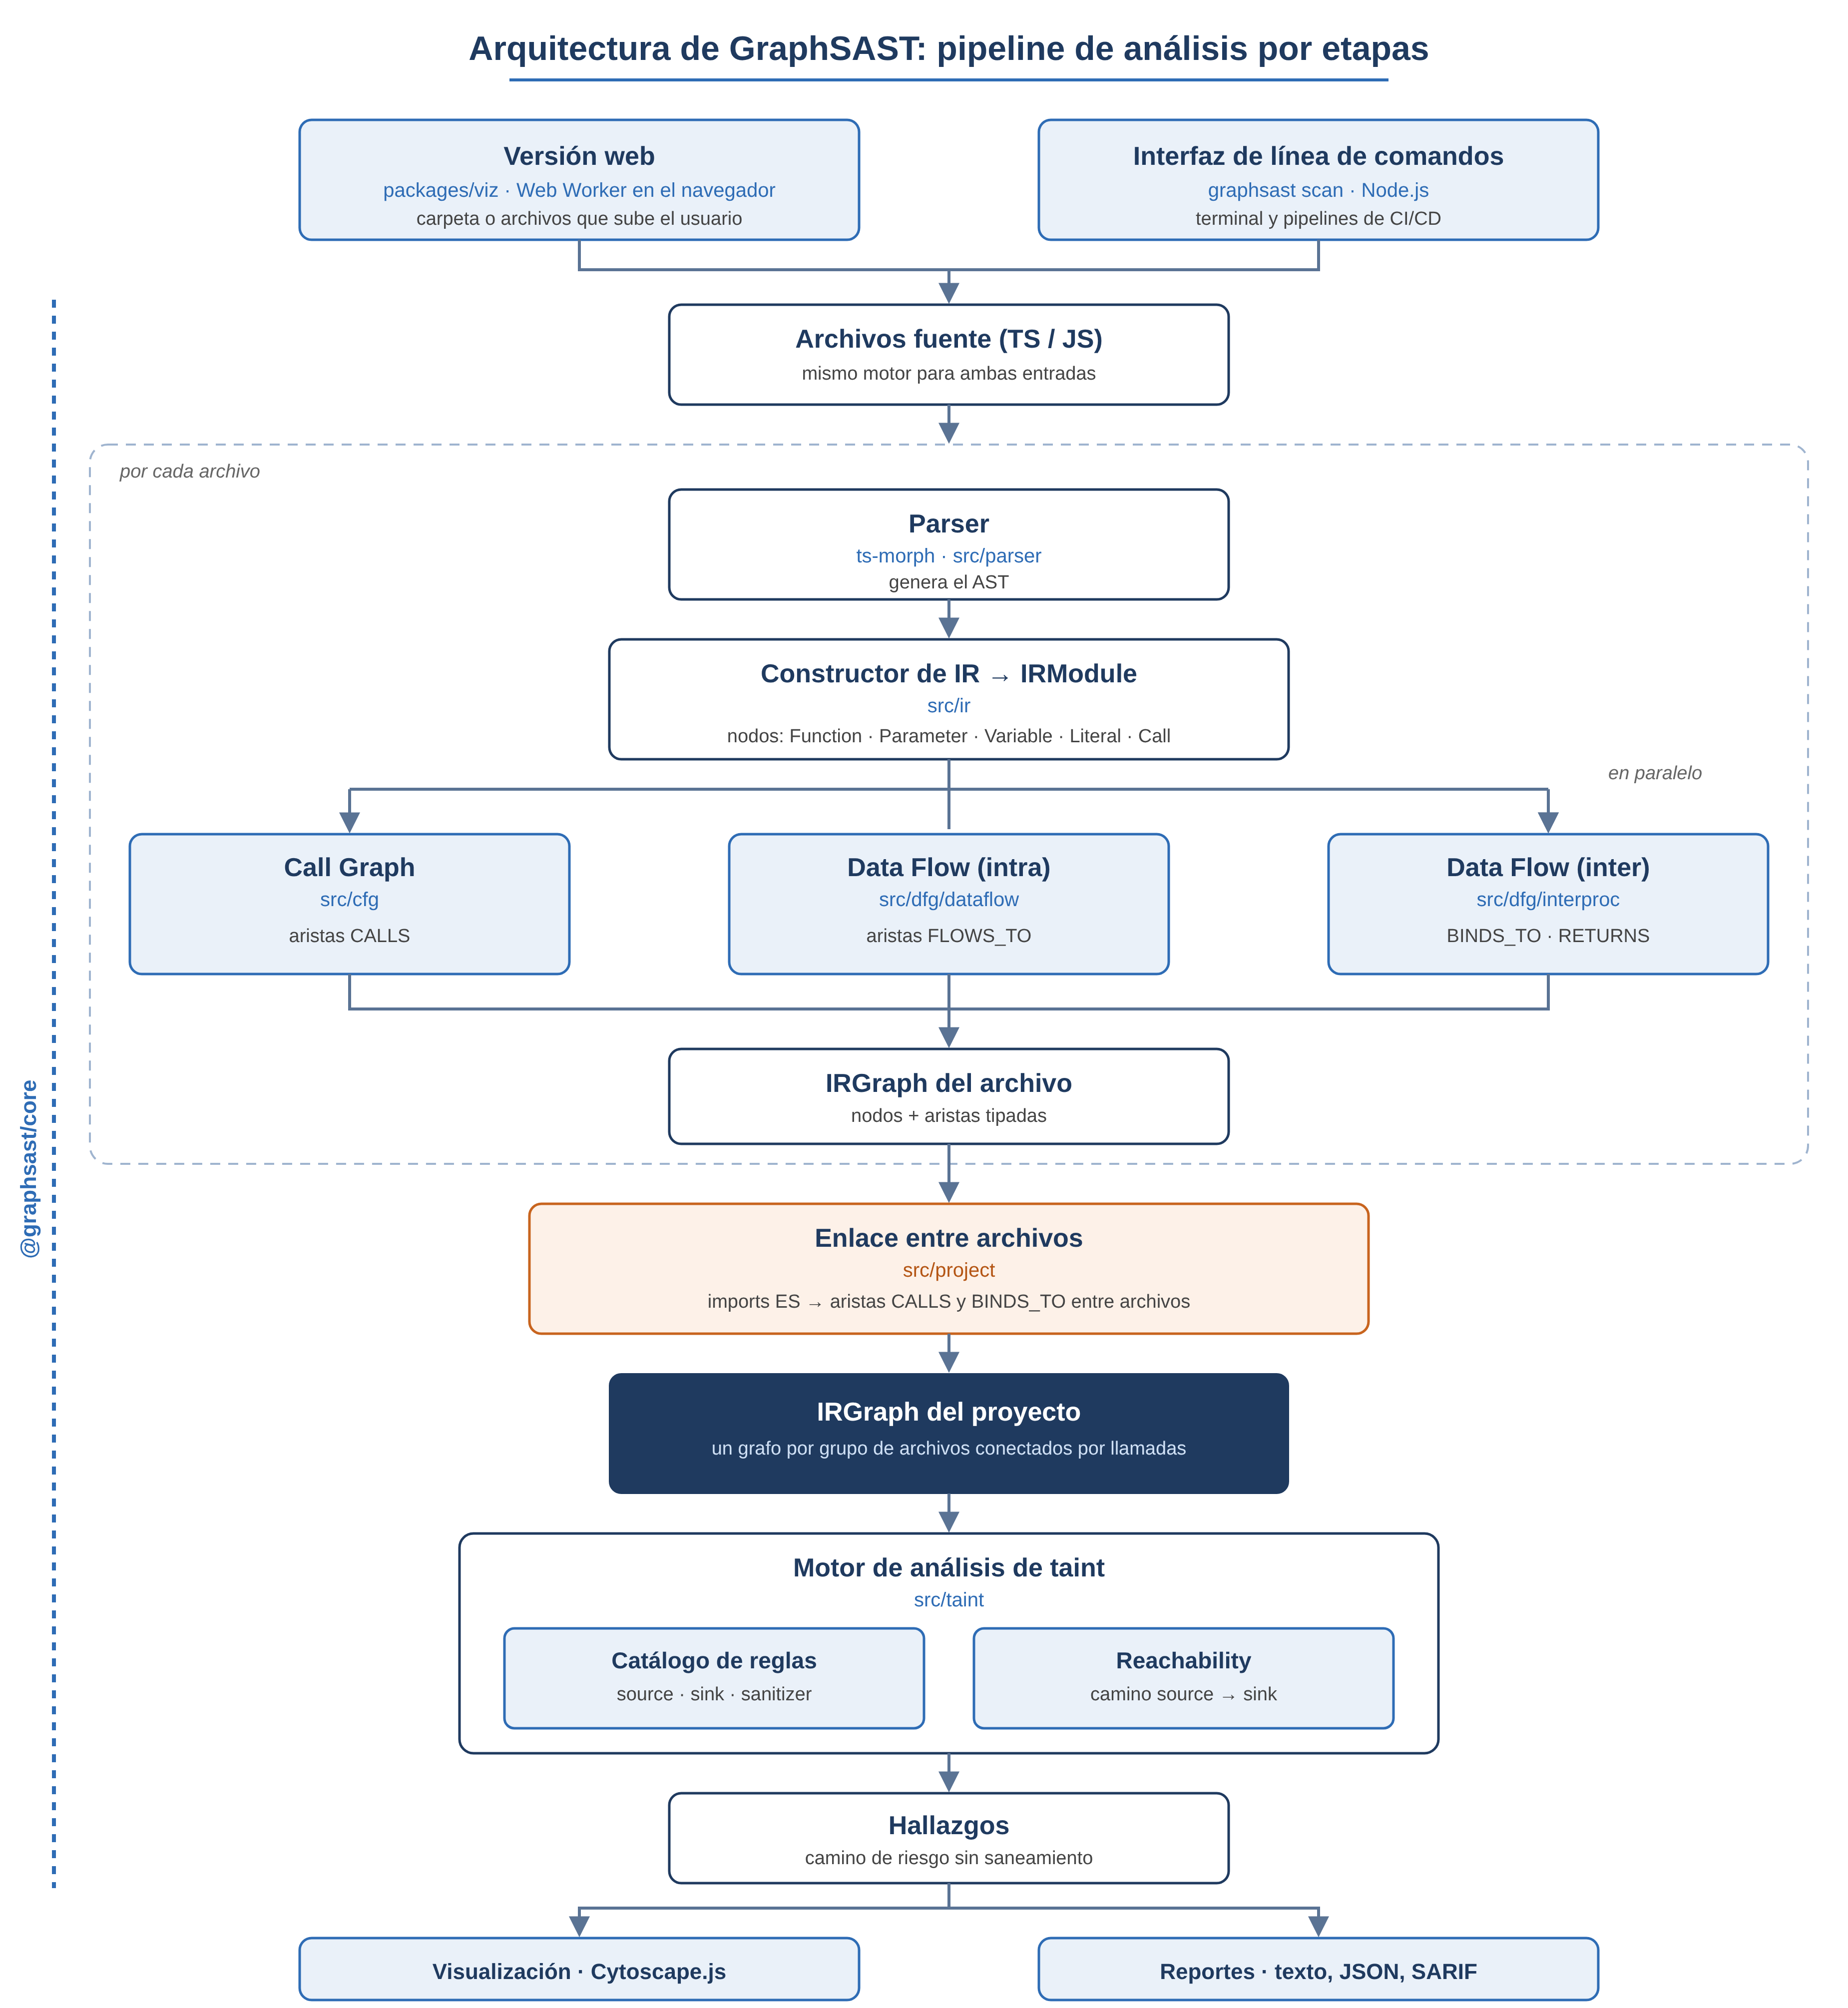
\includegraphics[width=0.7\textwidth]{figuras/arquitectura.png}
    \caption{Arquitectura de GraphSAST: pipeline de análisis por etapas, desde los archivos del proyecto hasta la visualización y los reportes, con enlace entre archivos}
    \label{fig:arquitectura}
\end{figure}

\section{Prototipo y alcance de lo construido}\label{sec:n4.2}

\subsection{Estado del desarrollo}\label{sec:n4.2.1}

El sistema se encuentra actualmente en estado de prototipo funcional. Se ejecuta como aplicación web en el navegador y procesa de forma satisfactoria los casos de prueba, aunque su alcance se define como prototipo y no como producto mínimo viable, ya que aún no fue evaluado por usuarios externos y ciertas características necesarias para su comercialización, como la gestión de suscripciones, forman parte de etapas futuras.

\subsection{Funcionalidades implementadas}\label{sec:n4.2.2}

El prototipo ejecuta el pipeline completo de análisis sobre los archivos de un proyecto: análisis sintáctico, construcción de la representación intermedia, generación del grafo de llamadas, análisis de flujo de datos intra e inter-procedural, y detección de recorridos desde puntos de entrada hacia operaciones sensibles sin saneamiento intermedio. La detección se resuelve mediante dos motores intercambiables: un recorrido en anchura sobre el grafo en memoria, empleado por defecto, y una consulta declarativa en Cypher ejecutada sobre el grafo persistido en Neo4j, que descarta los caminos que atraviesan un nodo de saneamiento y acota la profundidad de búsqueda. Los resultados se presentan mediante visualización interactiva del grafo, con resaltado del camino de riesgo y vinculación con las líneas de código correspondientes. El análisis sigue el dato de un archivo a otro cuando una función importada desde otro archivo del proyecto lo recibe como argumento. La versión web analiza una carpeta o un conjunto de archivos elegidos por el usuario, y la interfaz de línea de comandos analiza rutas del disco, emite reportes en texto, JSON y SARIF, y devuelve códigos de salida que permiten detener un pipeline de integración continua cuando se detectan hallazgos.

\subsection{Catálogo de detección}\label{sec:n4.2.3}

Se implementaron las tres debilidades definidas en el diseño arquitectónico, seleccionadas por constituir la tríada canónica del análisis de contaminación y por integrar el listado de debilidades más críticas publicado por MITRE, a las que se sumó la inyección NoSQL (CWE-943), habitual en aplicaciones Node.js que emplean bases de datos documentales como MongoDB:

\begin{table}[H]
    \centering
    \caption{Debilidades cubiertas por el catálogo de detección implementado}
    \label{tab:catalogo}
    \small
    \begin{tabularx}{\textwidth}{l L r r}
        \toprule
        \tb{Debilidad} & \tb{Descripción} & \tb{Sinks} & \tb{Sanitizers} \\
        \midrule
        CWE-89 & Inyección SQL & 5 & 5 \\
        CWE-78 & Inyección de comandos del sistema operativo & 6 & 4 \\
        CWE-79 & Cross-Site Scripting (XSS) & 6 & 5 \\
        CWE-943 & Inyección NoSQL & 6 & 4 \\
        \bottomrule
    \end{tabularx}
\end{table}

Las operaciones sensibles registradas corresponden a llamadas habituales del ecosistema analizado: controladores de bases de datos relacionales, mapeadores objeto-documento, ejecución de procesos del sistema operativo y manipulación del modelo de objetos del documento. Las operaciones de saneamiento reconocidas comprenden tanto funciones genéricas de validación y escapado como bibliotecas específicas del dominio.

\subsection{Verificación y resultados}\label{sec:n4.2.4}

El desarrollo cuenta con una suite de pruebas automatizadas organizadas según la etapa del pipeline que verifican, lo que permite validar cada componente de forma aislada. La aplicación incorpora asimismo dos casos de demostración que difieren en una sola línea: un fragmento en el que el identificador recibido en la URL cruza de una función a otra y llega a una consulta a base de datos, y el mismo fragmento con una operación de saneamiento intermedia. Los demás escenarios, como los flujos dentro de una misma función, las operaciones sensibles alcanzadas por literales, las entradas de Express, la inyección de comandos y el XSS, se cubren en el banco de pruebas descrito más adelante.

La figura siguiente presenta el análisis de un caso vulnerable. El dato ingresa por el parámetro de una función, se asigna a una variable intermedia, se transfiere como argumento a otra función y alcanza una operación de consulta a base de datos sin haber atravesado ninguna operación de saneamiento. El sistema identifica el recorrido y lo resalta sobre el grafo, indicando además las líneas de código involucradas.

\begin{figure}[H]
    \centering
    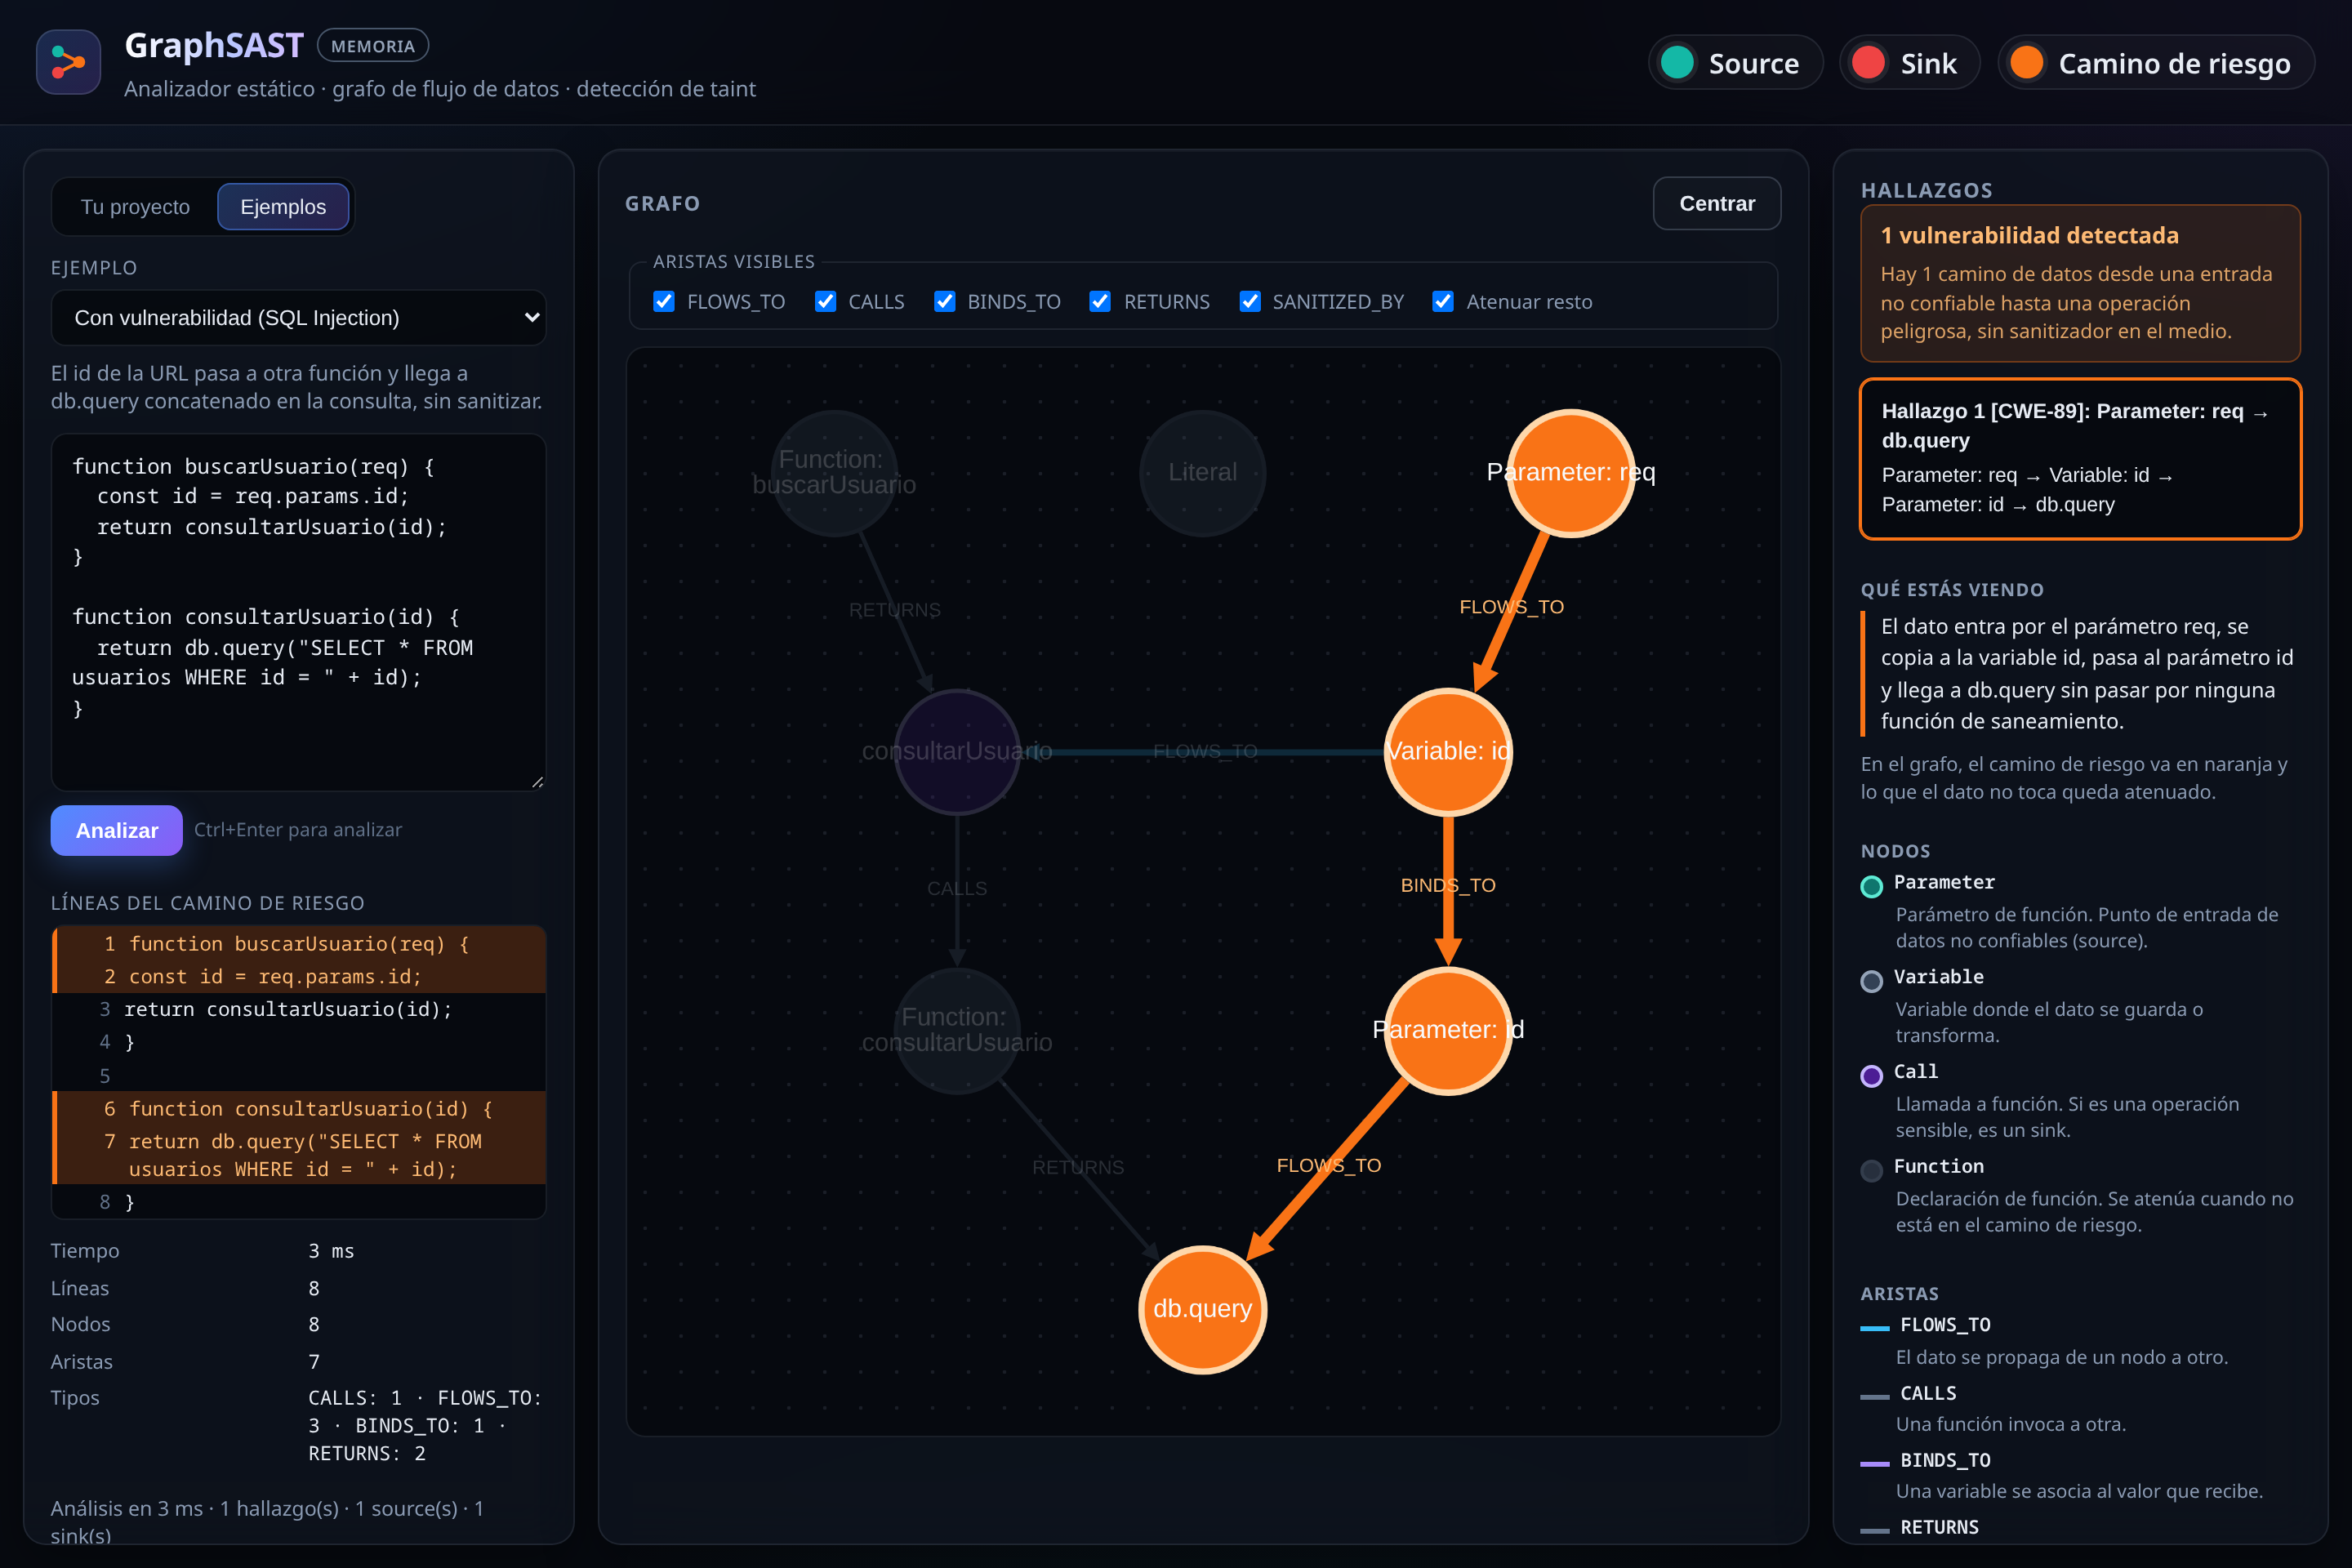
\includegraphics[width=0.9\textwidth]{figuras/deteccion.png}
    \caption{Detección de vulnerabilidad (CWE-89): el dato fluye desde el parámetro de entrada hasta la operación de consulta sin saneamiento intermedio. El camino de riesgo se resalta en la visualización}
    \label{fig:deteccion}
\end{figure}

El comportamiento ante un dato correctamente validado resulta particularmente relevante para las hipótesis del trabajo. En el caso siguiente, el mismo patrón de flujo incorpora una operación de saneamiento intermedia. El sistema reconoce la presencia de un punto de entrada y de una operación sensible —los identifica y los diferencia cromáticamente— pero descarta el hallazgo al verificar el saneamiento en el recorrido. Una herramienta basada en coincidencia de patrones señalaría la operación como vulnerable, dado que carece de la capacidad de determinar si el dato fue procesado en el trayecto.

\begin{figure}[H]
    \centering
    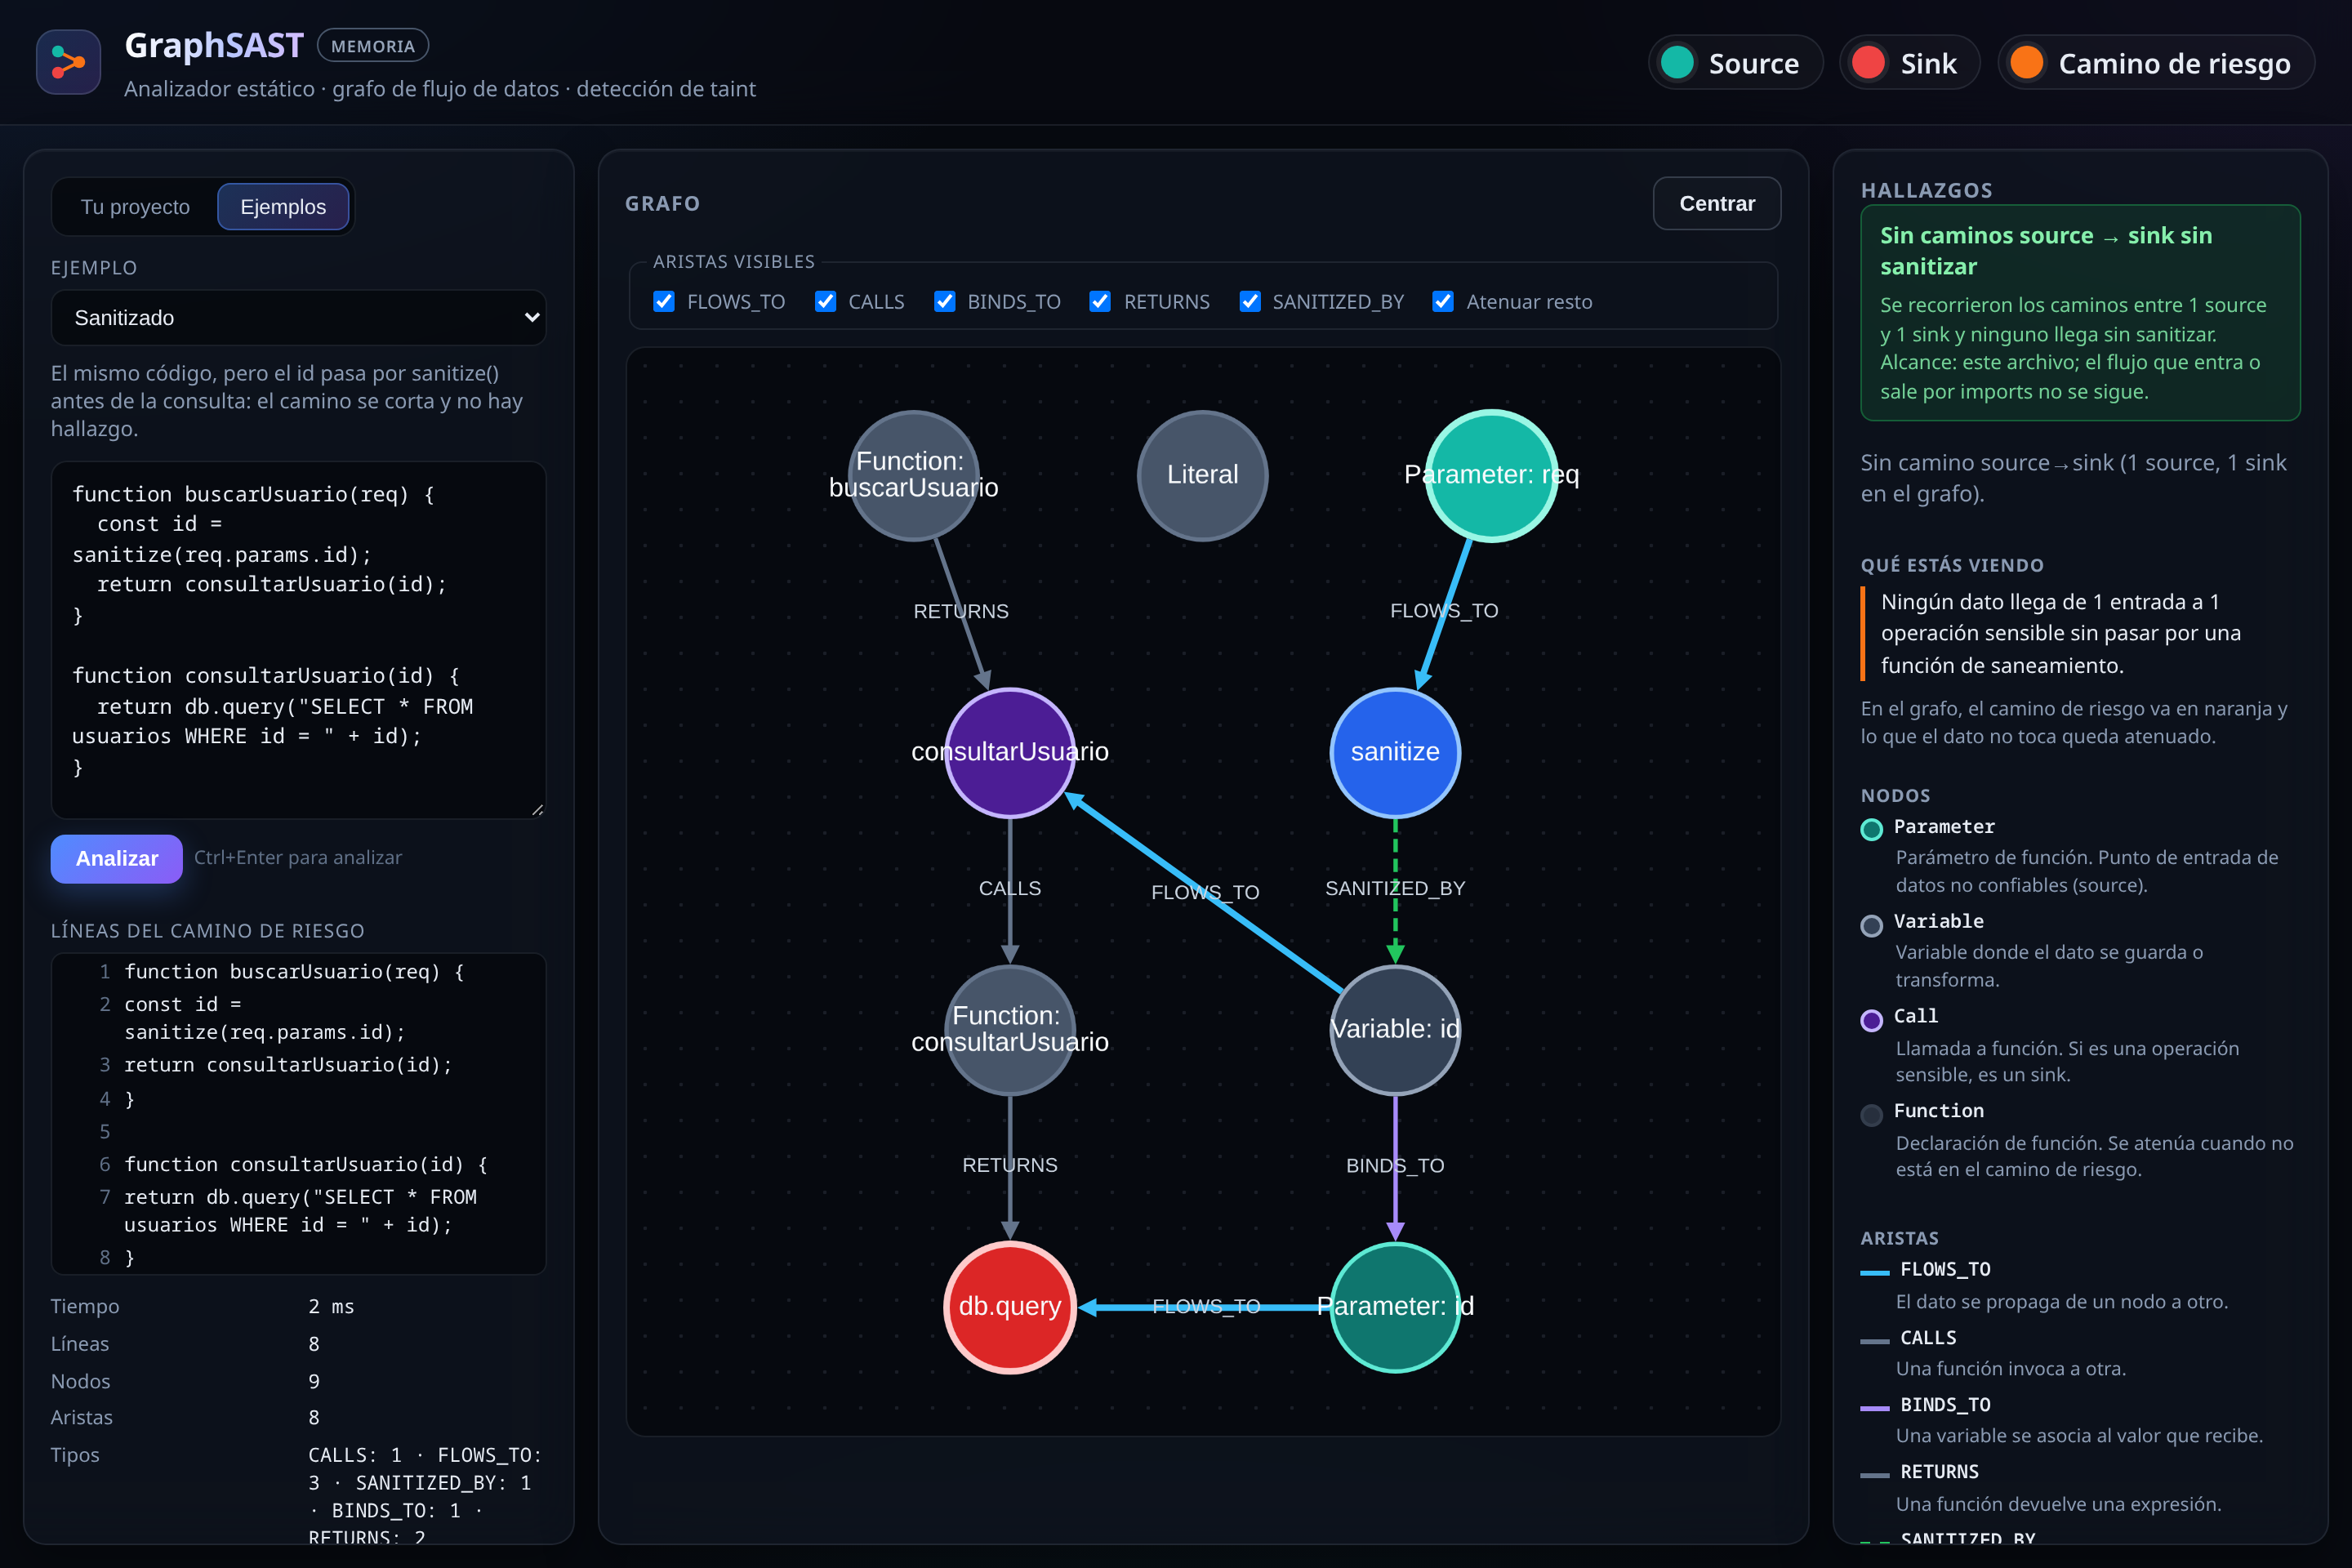
\includegraphics[width=0.9\textwidth]{figuras/saneado.png}
    \caption{Caso saneado: el mismo patrón de flujo con una operación de saneamiento intermedia. El sistema identifica el origen y el destino sensible, pero descarta el hallazgo al constatar el saneamiento en el recorrido}
    \label{fig:saneado}
\end{figure}

La interfaz expone asimismo las métricas correspondientes a cada ejecución, que incluyen el tiempo de análisis, la cantidad de líneas procesadas, y el número de nodos y aristas generados en el grafo, discriminados por tipo de relación. Los tiempos registrados sobre los casos de prueba se ubican en el orden de las decenas de milisegundos.

\begin{figure}[H]
    \centering
    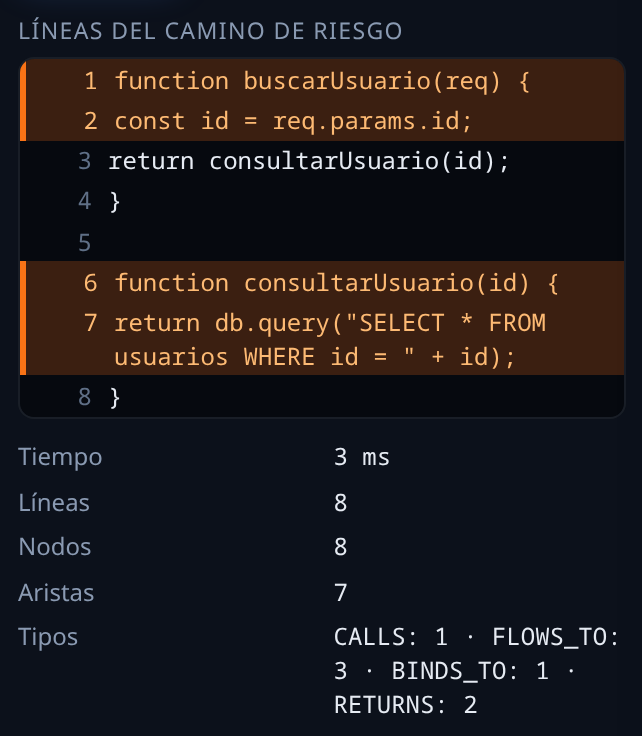
\includegraphics[width=0.5\textwidth]{figuras/metricas.png}
    \caption{Panel de métricas y líneas del camino de riesgo correspondientes al análisis ejecutado}
    \label{fig:metricas}
\end{figure}

La evaluación cuantitativa se ejecuta sobre un banco de pruebas etiquetado y reproducible desde la línea de comandos, integrado por cuarenta y tres casos de verdad conocida (veintinueve vulnerables y catorce seguros) que cubren recorridos intra e inter-procedurales, casos saneados, operaciones sensibles alcanzadas por literales constantes y entradas propias de Express. Además de las tres debilidades del catálogo, el banco incorpora casos de validación insuficiente de la entrada (CWE-20) que alcanzan operaciones sensibles ya catalogadas. Cada caso se clasifica de forma binaria según el sistema emita o no hallazgos, lo que permite construir la matriz de confusión y derivar los indicadores definidos en el Capítulo~\ref{cap:metodologia}.

\begin{table}[H]
    \centering
    \caption{Resultados del banco de pruebas sintético (43 casos; tiempos: mediana de cinco ejecuciones)}
    \label{tab:banco-sintetico}
    \small
    \begin{tabularx}{\textwidth}{L l}
        \toprule
        \tb{Indicador} & \tb{Valor obtenido} \\
        \midrule
        Verdaderos positivos (TP) & 29 \\
        Falsos positivos (FP) & 0 \\
        Verdaderos negativos (TN) & 14 \\
        Falsos negativos (FN) & 0 \\
        Precisión & 1,00 \\
        Exhaustividad (Recall) & 1,00 \\
        F1 & 1,00 \\
        Tiempo total de análisis & 52 ms \\
        Tiempo por línea de código & 0,27 ms \\
        \bottomrule
    \end{tabularx}
\end{table}

Corresponde delimitar el alcance de estos valores. Se obtienen sobre un corpus sintético reducido, construido por el propio autor y acotado a las construcciones sintácticas que el analizador cubre, por lo que no constituyen evidencia de desempeño sobre proyectos reales ni admiten generalización. Su función en esta instancia es la de una prueba de regresión que verifica que el motor no emite alertas sobre los casos correctamente saneados ni omite los recorridos vulnerables conocidos. La comparación cuantitativa con una herramienta de referencia, prevista en el diseño de investigación del Capítulo~\ref{cap:metodologia}, permanece pendiente. La validación frente a vulnerabilidades documentadas se presenta a continuación.

Para contrastar el sistema con vulnerabilidades reales se empleó un corpus de seis advisories del ecosistema npm publicados en la base de datos de advisories de GitHub, relevados el 1 de septiembre de 2026 y congelados para que la medición resulte reproducible, restringidos a las debilidades del catálogo. Para cada caso se descargan del registro de npm la versión vulnerable del paquete y la versión que corrige la falla, se analizan ambas contando solo los hallazgos de la debilidad del advisory y se registran dos resultados: si la versión vulnerable presenta hallazgos (detección) y si la corrección del mantenedor reduce su cantidad (discriminación). La discriminación constituye la evidencia fuerte, dado que indica que el hallazgo se vincula con la vulnerabilidad y no con un patrón presente en todo el paquete.

\begin{table}[H]
    \centering
    \caption{Validación sobre vulnerabilidades documentadas del ecosistema npm (6 casos)}
    \label{tab:advisories}
    \footnotesize
    \begin{tabularx}{\textwidth}{>{\hsize=1.3\hsize}L r l r c >{\hsize=.7\hsize}L}
        \toprule
        \tb{Paquete (vulnerable $\rightarrow$ corregida)} & \tb{CWE} & \tb{Advisory} & \tb{Archivos} & \tb{\makecell{Hallazgos\\(vuln. $\rightarrow$ corr.)}} & \tb{Resultado} \\
        \midrule
        @hypequery/clickhouse 2.5.0 $\rightarrow$ 2.5.1 & 89 & GHSA-6wcc-39rp-hh9p & 0 & — & Sin código fuente publicado \\
        @anthropic-ai/claude-code 2.1.162 $\rightarrow$ 2.1.163 & 78 & GHSA-7835-87q9-rgvv & 3 & 0 $\rightarrow$ 0 & No detectado \\
        sanitize-html 2.17.4 $\rightarrow$ 2.17.5 & 79 & GHSA-vccv-cmxp-4j9h & 1 & 0 $\rightarrow$ 0 & No detectado \\
        sanitize-html 2.17.6 $\rightarrow$ 2.17.7 & 79 & GHSA-g8qq-57p8-ggw5 & 1 & 0 $\rightarrow$ 0 & No detectado \\
        defuddle 0.19.0 $\rightarrow$ 0.19.1 & 79 & GHSA-jg4p-g6xj-4qmf & 0 & — & Sin código fuente publicado \\
        dompurify 3.4.12 $\rightarrow$ 3.4.13 & 79 & GHSA-55q2-fjhq-7xh7 & 7 & 1 $\rightarrow$ 1 & Detectado, sin discriminación \\
        \bottomrule
    \end{tabularx}
\end{table}

El sistema detectó uno de los seis casos (16,7 \%) y ninguno con discriminación: el único hallazgo, en DOMPurify, se mantiene en la versión corregida, por lo que no corresponde a la vulnerabilidad reportada. El análisis de los casos explica el resultado. En dos paquetes, @hypequery/clickhouse y defuddle, el registro de npm solo contiene código compilado en la carpeta dist, que el evaluador excluye por tratarse de código generado; como verificación complementaria se analizó también esa carpeta, sin cambios en la conclusión: ningún hallazgo en el primero y tres hallazgos idénticos en ambas versiones del segundo. El paquete de @anthropic-ai/claude-code publica únicamente un envoltorio de instalación. En cuanto a la naturaleza de las fallas, las de sanitize-html y DOMPurify residen en la lógica interna de esas bibliotecas de saneamiento, como la validación incompleta de esquemas de URI o la eliminación de nodos del documento, y consisten en omisiones de sus propias reglas de filtrado; la de @hypequery/clickhouse es un error en su función de escapado de parámetros; la de defuddle consiste en interpolar atributos sin escapar al construir HTML como texto, una operación que el catálogo no registra como destino sensible; y la de inyección de comandos se origina en una confusión de rutas que habilita el escape del entorno aislado. Ninguna adopta la forma de un recorrido desde una entrada no confiable hasta una operación sensible del catálogo, que es la clase de vulnerabilidad que el modelo de accesibilidad detecta.

En consecuencia, esta validación no permite afirmar la efectividad del sistema sobre código real, y tampoco la refuta: el corpus se compone de bibliotecas cuyas fallas quedan fuera del modelo de amenaza del analizador. La validación pendiente debe orientarse a aplicaciones que reciben entradas de usuario y las conducen hacia bases de datos, procesos del sistema o el documento, que es el escenario para el que la herramienta fue diseñada, y ampliar la cantidad de casos hasta admitir conclusiones cuantitativas.

\subsection{Limitaciones del alcance actual}\label{sec:n4.2.5}

\paragraph{Alcance del análisis entre archivos.} El dato se sigue de un archivo a otro cuando un archivo invoca una función declarada con function en otro archivo del proyecto e importada mediante import de módulos ES con ruta relativa. No se siguen las importaciones mediante require, las funciones flecha o asignadas a constantes, los métodos de clase, los alias de rutas de TypeScript ni los paquetes de terceros; en esos casos cada archivo se analiza por separado. Por la misma razón, las aplicaciones organizadas en clases o con funciones flecha, habituales en Express y NestJS, quedan cubiertas de forma parcial.

\paragraph{Motor de consultas por defecto.} El sistema implementa los dos motores de resolución previstos en el diseño arquitectónico: el recorrido en memoria y la consulta declarativa en Cypher sobre el grafo persistido en Neo4j. El motor sobre base de datos opera, no obstante, de manera opcional, dado que requiere una instancia activa y la configuración de la variable de entorno correspondiente; en ausencia de dicha instancia la aplicación recurre al recorrido en memoria, que constituye el modo de operación por defecto. La paridad entre ambos motores se verificó sobre casos sintéticos y no sobre proyectos de escala.

\paragraph{Validación con usuarios.} No se realizaron pruebas de usabilidad con usuarios externos, instancia requerida para la validación de la hipótesis relativa a la utilidad de la visualización.

\subsection{Próximos pasos}\label{sec:n4.2.6}

Se prevé la consolidación del motor sobre base de datos de grafos como modo de operación habitual, la ampliación del catálogo de reglas y de los patrones de llamada que resuelve el análisis entre archivos, y la integración de la interfaz de línea de comandos en pipelines de integración continua como complemento de la versión web. Esta modalidad resulta coherente con el enfoque de incorporación temprana de controles de seguridad que fundamenta el proyecto: el análisis puede ejecutarse de forma automática sobre cada cambio del código, y en ambas modalidades el código fuente no abandona la infraestructura del usuario.

\section{Stack de software}\label{sec:n4.3}

La selección de tecnologías respondió a criterios explícitos de viabilidad, adecuación al dominio y coherencia interna del stack. La tabla siguiente resume las herramientas empleadas y la capa en la que interviene cada una.

\begin{table}[H]
    \centering
    \caption{Tecnologías empleadas en el desarrollo del prototipo}
    \label{tab:stack}
    \small
    \begin{tabularx}{\textwidth}{l l l L}
        \toprule
        \tb{Tecnología} & \tb{Versión} & \tb{Capa} & \tb{Función} \\
        \midrule
        TypeScript & 5.5 & Transversal & Lenguaje del motor y de la interfaz \\
        Node.js & — & Entorno de ejecución & Ejecución del motor de análisis \\
        Web Workers & — & Ejecución & Análisis en segundo plano en el navegador \\
        ts-morph & 23.0 & Análisis sintáctico & Generación y recorrido del AST \\
        Cytoscape.js & 3.30 & Visualización & Renderizado interactivo del grafo \\
        Vite & 5.4 & Construcción & Empaquetado y servidor de desarrollo \\
        Vitest & 2.0 & Pruebas & Ejecución de la suite automatizada \\
        npm workspaces & — & Estructura & Gestión del monorepo \\
        Neo4j & 5 Community & Persistencia & Almacenamiento del grafo compilado \\
        neo4j-driver & 6.2 & Persistencia & Cliente Bolt y ejecución de consultas Cypher \\
        Docker Compose & — & Entorno & Provisión local de la instancia de Neo4j \\
        Vercel & — & Despliegue & Publicación de la aplicación web como sitio estático \\
        \bottomrule
    \end{tabularx}
\end{table}

\subsection{Estrategia de análisis sintáctico}\label{sec:n4.3.1}

Se decidió utilizar la biblioteca ts-morph en lugar de programar un analizador sintáctico propio. Desarrollar un parser completo para la gramática de TypeScript y sus continuas actualizaciones habría consumido gran parte del tiempo del proyecto sin aportar valor diferencial. El aporte de GraphSAST está en los algoritmos de construcción del grafo de flujo de datos, el análisis de taint y la visualización del riesgo.

ts-morph simplifica la interacción con el compilador oficial de TypeScript y expone una API clara para recorrer los nodos del AST, lo que reduce de manera considerable el código necesario para navegar la estructura del programa.

\subsection{Lenguaje del motor}\label{sec:n4.3.2}

El motor se implementó en TypeScript sobre Node.js. La elección responde a tres razones: permite emplear un único lenguaje a lo largo de todo el sistema, incluida la interfaz de visualización; el sistema de tipos resulta adecuado para modelar las estructuras del grafo, en las que la distinción entre categorías de nodos y de aristas es central; y el ecosistema ofrece acceso directo a las herramientas de análisis del lenguaje objetivo. Se descartó el uso de Python, dado que el tratamiento del árbol sintáctico de TypeScript resulta menos natural fuera de su propio ecosistema, así como una solución híbrida que combinara ambos entornos, por la complejidad operativa que introduciría.

\subsection{Visualización}\label{sec:n4.3.3}

La representación gráfica se implementó con Cytoscape.js, una biblioteca JavaScript orientada específicamente a la construcción y visualización interactiva de grafos en el navegador. La selección se fundamentó en un relevamiento de herramientas del área y en la consulta con desarrolladores con experiencia previa en la materia. Se consideraron asimismo Gephi e igraph, descartadas por no resultar integrables en una aplicación web: la primera constituye una aplicación de escritorio orientada a la exploración manual de grafos, y la segunda una biblioteca de análisis destinada al cómputo de métricas antes que al renderizado interactivo. Cytoscape.js provee de manera nativa los algoritmos de disposición y el modelo de nodos y aristas requeridos por el proyecto, y cuenta con adopción consolidada en contextos de investigación y análisis de grafos.

\subsection{Herramientas de construcción y pruebas}\label{sec:n4.3.4}

El módulo de visualización emplea Vite como empaquetador y servidor de desarrollo. La elección respondió a la experiencia previa con la herramienta en proyectos de características similares, criterio que reduce la curva de aprendizaje y el riesgo de configuración en un desarrollo acotado en el tiempo. Vite ofrece además soporte nativo para TypeScript y módulos ES, lo que resulta coherente con el resto del stack. Las pruebas automatizadas se ejecutan con Vitest, seleccionado por su integración directa con Vite y por compartir su configuración, evitando duplicar la infraestructura de construcción del proyecto.

\section{Infraestructura y modelo de ejecución}\label{sec:n4.4}

El sistema se distribuye como una aplicación web estática: el servidor entrega la página y el análisis se ejecuta en el navegador del usuario. No se estructura como un servicio con procesamiento en el servidor, y esta característica condiciona los requerimientos de infraestructura, que difieren de los correspondientes a un servicio alojado convencional.

\subsection{Modelo de ejecución}\label{sec:n4.4.1}

El usuario accede a la aplicación desde el navegador y selecciona la carpeta o los archivos de su proyecto. El motor de análisis, el mismo que utiliza la interfaz de línea de comandos, se ejecuta en un proceso en segundo plano del navegador (Web Worker), de modo que la interfaz permanece operativa durante el análisis. Los archivos se leen y se analizan en el equipo del usuario: el servidor de alojamiento solo entrega los archivos estáticos de la aplicación y no recibe el código analizado. Esta propiedad resulta pertinente al dominio del proyecto: dado que la herramienta procesa código fuente potencialmente sensible, el hecho de que dicho código no abandone el entorno del usuario constituye una garantía relevante. La interfaz de línea de comandos, que ejecuta el mismo motor sobre Node.js, se mantiene para su uso en terminal y en pipelines de integración continua.

\subsection{Requerimientos}\label{sec:n4.4.2}

La versión web requiere únicamente un navegador actualizado; la interfaz de línea de comandos requiere un entorno con Node.js. No se requiere hardware especializado, servicios de terceros ni infraestructura de servidores. El desarrollo y las pruebas se realizaron sobre un equipo de escritorio de características estándar.

\subsection{Disponibilidad y escalabilidad}\label{sec:n4.4.3}

Al ejecutarse el análisis en el navegador de cada usuario, el servidor no realiza procesamiento y la carga de cada análisis recae en el equipo que lo solicita, por lo que la disponibilidad y la escalabilidad se reducen a la entrega de archivos estáticos. El factor determinante del rendimiento es el tamaño del código analizado, dado que el costo computacional del análisis crece con la cantidad de nodos y aristas del grafo generado. Como referencia, en el equipo de desarrollo el análisis en el navegador de un proyecto de 78 archivos y unas 8.500 líneas demandó alrededor de 2,8 segundos. La caracterización de dicho crecimiento forma parte de las mediciones previstas en la validación del sistema.

\section{Modelo de datos: el grafo del programa}\label{sec:n4.5}

El sistema representa el programa analizado mediante un grafo dirigido en el que los nodos corresponden a los elementos por los que circula la información y las aristas a las relaciones que se establecen entre ellos. Este modelo constituye el núcleo del aporte técnico del trabajo, dado que sobre él se resuelve la detección de vulnerabilidades.

\subsection{Nodos}\label{sec:n4.5.1}

Se definen cinco categorías de nodo. Cada nodo almacena su ubicación exacta en el código fuente —archivo, línea y columna— junto con el fragmento de texto correspondiente, lo que permite vincular cualquier elemento del grafo con su posición original en el programa.

\begin{table}[H]
    \centering
    \caption{Categorías de nodo del modelo de grafo}
    \label{tab:nodos}
    \small
    \begin{tabularx}{\textwidth}{l L}
        \toprule
        \tb{Categoría} & \tb{Elemento representado} \\
        \midrule
        Function & Declaración de función \\
        Parameter & Parámetro de entrada de una función \\
        Variable & Variable declarada \\
        Literal & Valor literal presente en el código \\
        Call & Invocación a una función u operación \\
        \bottomrule
    \end{tabularx}
\end{table}

\subsection{Aristas}\label{sec:n4.5.2}

Se definen cinco categorías de relación dirigida. La distinción entre categorías resulta determinante para el funcionamiento del sistema, dado que permite diferenciar la propagación efectiva de un valor de otras relaciones estructurales del programa.

\begin{table}[H]
    \centering
    \caption{Categorías de relación del modelo de grafo}
    \label{tab:aristas}
    \small
    \begin{tabularx}{\textwidth}{l L}
        \toprule
        \tb{Relación} & \tb{Significado} \\
        \midrule
        CALLS & Una función invoca a otra \\
        FLOWS\_TO & Un valor se propaga de un nodo a otro \\
        BINDS\_TO & Una variable se asocia al valor que recibe \\
        RETURNS & Una función devuelve una expresión \\
        SANITIZED\_BY & Un valor atraviesa una operación de saneamiento \\
        \bottomrule
    \end{tabularx}
\end{table}

\subsection{Resolución de la detección sobre el modelo}\label{sec:n4.5.3}

La identificación de una vulnerabilidad se resuelve como un problema de accesibilidad sobre el grafo: se determina si existe un camino que conecte un nodo de origen con un nodo de destino sensible sin que dicho recorrido atraviese una relación de saneamiento. Esta formulación traduce el planteo conceptual del trabajo —la seguridad entendida como accesibilidad sobre un grafo dirigido— en una operación computable sobre una estructura de datos concreta.

La relación de saneamiento cumple un rol central para evitar falsas alarmas: si una variable fue validada en el trayecto, el sistema descarta el camino. Un analizador basado en coincidencia de patrones carece de esa información y debe reportar el caso como potencialmente vulnerable.

Durante la implementación de las consultas Cypher sobre Neo4j surgió una dificultad concreta con las llamadas recursivas o cíclicas entre funciones, que generaban recorridos de longitud indefinida y demoraban el motor. Para resolverlo se acotó la profundidad de búsqueda a quince saltos entre el origen y el destino. En el recorrido en memoria ese límite es el valor por defecto de un parámetro configurable, mientras que en la consulta Cypher queda fijado en el patrón de camino. La restricción evita los recorridos indefinidos sin comprometer la detección en los flujos habituales de una aplicación web: sobre el banco de pruebas de 43 casos, el análisis completo demandó alrededor de 52 ms, aproximadamente 0,27 ms por línea de código (tabla~\ref{tab:banco-sintetico}).

\section{Diseño e interacción}\label{sec:n4.6}

\subsection{Usuario destinatario}\label{sec:n4.6.1}

La herramienta está orientada a desarrolladores y analistas que requieren auditar código fuente. El diseño asume familiaridad técnica con el lenguaje analizado y con los conceptos de seguridad involucrados, por lo que privilegia la densidad informativa sobre la simplificación de la interfaz.

\subsection{Organización de la interfaz}\label{sec:n4.6.2}

La aplicación se estructura en tres paneles simultáneos. El panel izquierdo ofrece dos modos. En el modo de proyecto, el usuario elige o arrastra una carpeta o un conjunto de archivos; la aplicación informa cuántos archivos se analizan y por qué se excluyen los demás, muestra el progreso del análisis y, al finalizar, lista los archivos con su cantidad de hallazgos junto con el contenido del archivo elegido y las líneas del camino de riesgo resaltadas (figura~\ref{fig:web-proyecto}). En el modo de ejemplos, el usuario puede ingresar un fragmento mediante un editor de texto o seleccionar uno de los dos ejemplos precargados: un fragmento con una inyección SQL y el mismo fragmento con una operación de saneamiento. El panel central presenta el grafo generado. El panel de hallazgos expone el veredicto, cada hallazgo con su debilidad, su ubicación y su recorrido, el catálogo de debilidades cubiertas y las reglas activas. La disposición simultánea responde a un criterio explícito: permitir que el usuario contraste el código, su representación como grafo y los hallazgos sin necesidad de alternar entre vistas.

\begin{figure}[H]
    \centering
    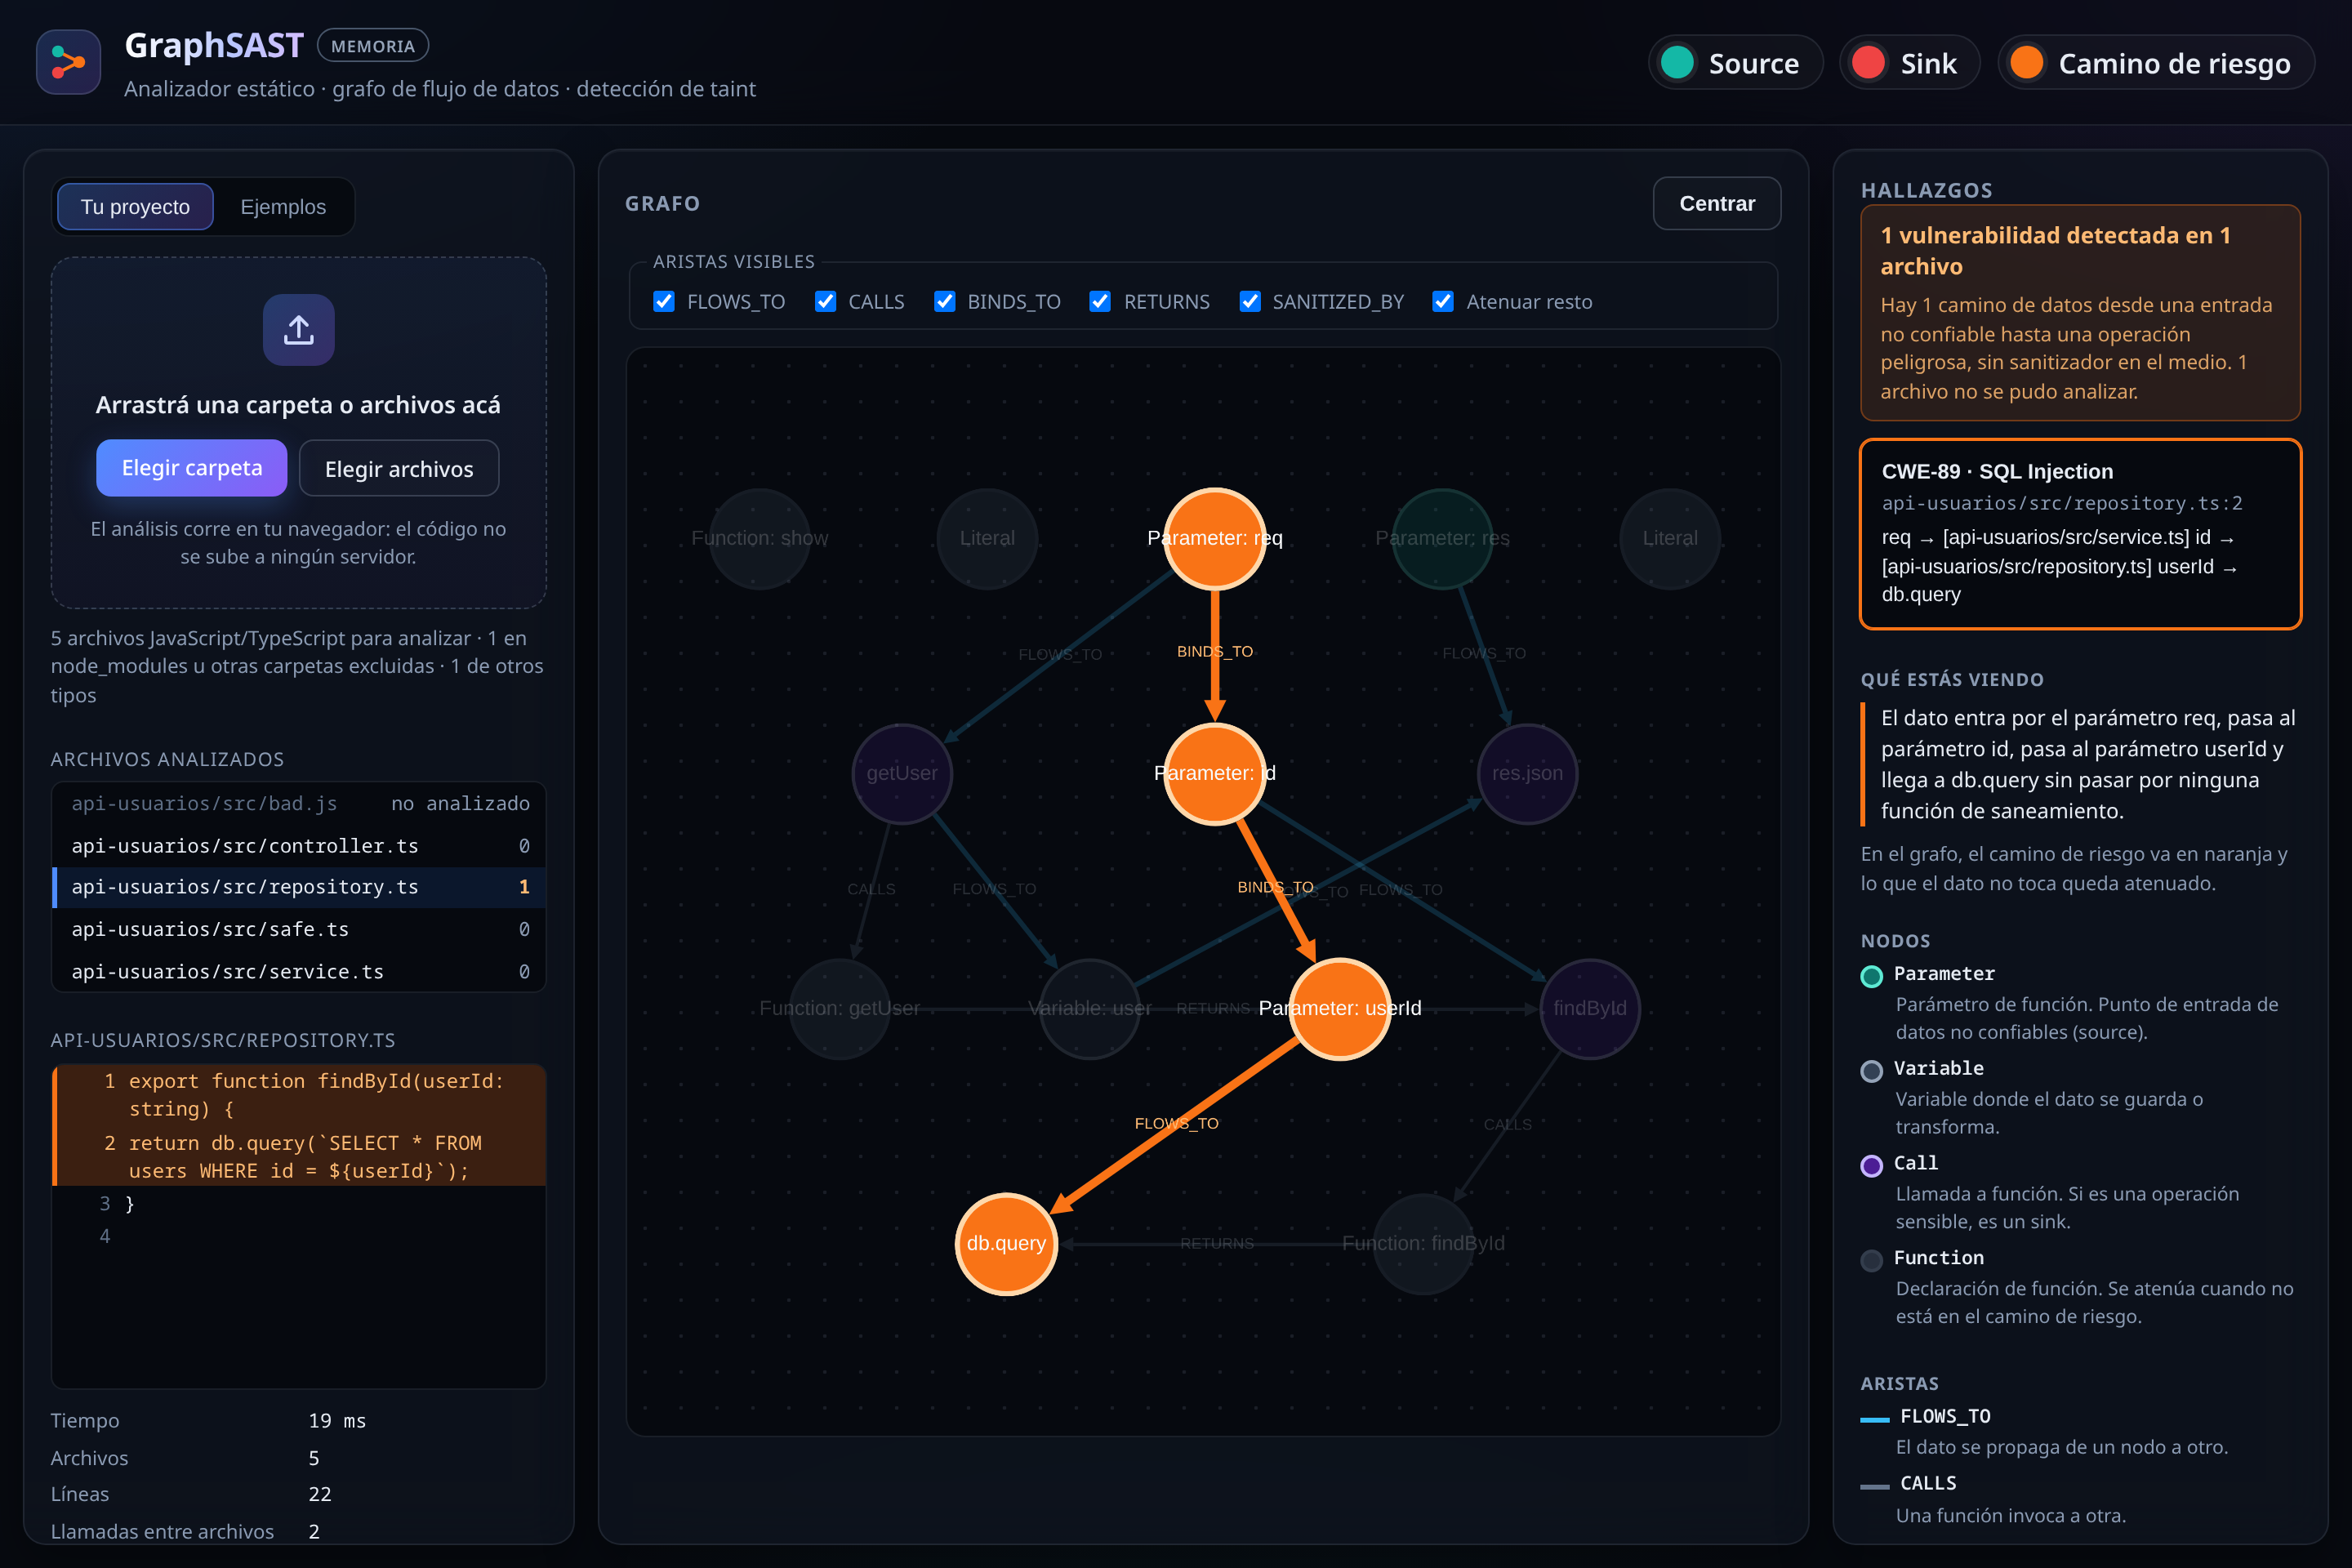
\includegraphics[width=0.9\textwidth]{figuras/web-proyecto.png}
    \caption{Versión web: análisis de un proyecto subido como carpeta. El hallazgo cruza tres archivos y se muestra el archivo del sink con las líneas del camino resaltadas}
    \label{fig:web-proyecto}
\end{figure}

\subsection{Decisiones de diseño}\label{sec:n4.6.3}

Se incorporó una codificación cromática con leyenda visible que distingue los nodos de origen, los nodos correspondientes a operaciones sensibles y el camino de riesgo identificado. Esta codificación permite interpretar el resultado de un análisis sin recurrir al texto: el contraste entre las figuras~\ref{fig:deteccion} y~\ref{fig:saneado} ilustra la diferencia entre un recorrido vulnerable y uno saneado a partir del color de los nodos y de las aristas.

El grafo admite el filtrado independiente de cada categoría de arista, junto con una opción de atenuación del resto de la estructura. Esta decisión atiende a un problema concreto de legibilidad: la superposición de relaciones de distinta naturaleza dificulta la lectura del recorrido relevante, por lo que el control sobre qué relaciones se muestran resulta necesario para interpretar grafos de cierto tamaño.

La interfaz señala además de manera explícita el modo de operación del motor mediante un indicador en el encabezado. En la versión web el análisis se resuelve siempre mediante el recorrido en memoria, dado que se ejecuta en el navegador; la consulta Cypher sobre el grafo persistido en Neo4j queda disponible a través de la API local. Esta decisión responde al criterio de que las condiciones de ejecución y las limitaciones del prototipo resulten visibles para el usuario.

\subsection{Vinculación con el código fuente}\label{sec:n4.6.4}

La interfaz presenta las líneas de código correspondientes al camino de riesgo detectado, y la selección de un nodo del grafo despliega su información asociada, incluida su ubicación en el archivo. Esta correspondencia entre la representación abstracta y el código concreto constituye el aspecto central del diseño, dado que la utilidad de la visualización depende de que el usuario pueda trasladar el hallazgo a una acción sobre el código.

\subsection{Accesibilidad y validación}\label{sec:n4.6.5}

Se incorporaron etiquetas descriptivas en los controles de la interfaz y regiones de actualización dinámica anunciables por lectores de pantalla, así como un atajo de teclado para ejecutar el análisis. No se realizaron pruebas de usabilidad con usuarios externos. La validación de la hipótesis relativa a la utilidad de la visualización requiere dicha instancia, prevista como trabajo posterior mediante sesiones de evaluación con desarrolladores.

\section{Calidad, seguridad y despliegue}\label{sec:n4.7}

\subsection{Estrategia de pruebas}\label{sec:n4.7.1}

El proyecto cuenta con una suite de pruebas automatizadas ejecutadas mediante Vitest. Las pruebas se organizan siguiendo la estructura por etapas del sistema, verificando de forma independiente el análisis sintáctico, la construcción de la representación intermedia, el grafo de llamadas, el análisis de flujo de datos, el motor de contaminación, la carga del catálogo de reglas, la generación de sentencias Cypher, la selección de motor, la construcción de informes, el análisis entre archivos y la carga de archivos de la versión web, además del módulo de visualización. La suite comprende doscientas cuarenta y siete pruebas distribuidas en veintisiete archivos. Esta organización deriva directamente de la decisión arquitectónica adoptada: la separación en etapas permite verificar cada componente de manera aislada y localizar con precisión el origen de una falla.

De modo complementario a las pruebas unitarias, la aplicación incorpora casos de demostración que reproducen patrones habituales de código y verifican el comportamiento del sistema tanto ante recorridos vulnerables como ante recorridos correctamente saneados.

\subsection{Control de versiones}\label{sec:n4.7.2}

El desarrollo se gestiona mediante Git, con repositorio alojado en GitHub: \url{https://github.com/MaxiZk/graphsast}. Los cambios se incorporan una vez verificado que la suite de pruebas se ejecuta satisfactoriamente y que la aplicación opera conforme a lo esperado, criterio que mantiene el repositorio en un estado funcional a lo largo del desarrollo.

\subsection{Consideraciones de seguridad}\label{sec:n4.7.3}

El sistema no administra cuentas de usuario, credenciales ni bases de datos remotas, por lo que no requiere esquemas de autenticación ni cifrado de datos en reposo. Una decisión clave del modelo de ejecución es que el código fuente analizado nunca se transmite fuera de la computadora del usuario: aunque la aplicación se sirve desde un servidor, el análisis se realiza en el navegador. Tratándose de código que puede contener vulnerabilidades o lógica propietaria, esa ejecución local elimina el riesgo de filtración hacia servidores externos.

\subsection{Despliegue}\label{sec:n4.7.4}

La aplicación web se publica como sitio estático en la plataforma Vercel, en \url{https://graph-sast.vercel.app/}. Vercel compila el proyecto a partir del repositorio y sirve los archivos resultantes sin funciones de servidor; se verificó sobre el sitio publicado que el análisis no genera solicitudes hacia otros dominios, de modo que el código analizado no sale del navegador. Para el desarrollo local, la ejecución requiere la instalación de las dependencias mediante el gestor de paquetes y la puesta en marcha del servidor de desarrollo.
